本章采用 AIDC 八模块覆盖包，并用“价值量--收入确认--利润率--现金流--估值信用”的因果链审计每个环节。\textbf{算力与存储}决定理论上限，但昇腾 950DT 的晶圆制造、HBM 制造/基底、先进封装、良率和量产规模均未披露，A 股不能因为“国产算力”标签自动获得芯片或 HBM 供应商身份。即便某公司具备半导体设备、探针卡或材料能力，也必须先找到产品、制程、客户、认证、订单和经济性证据；本案对强一股份等问答的处理，就是把提问者的前提退回待验证，而不是当作公司确认。

\begin{figure}[htbp]
\centering
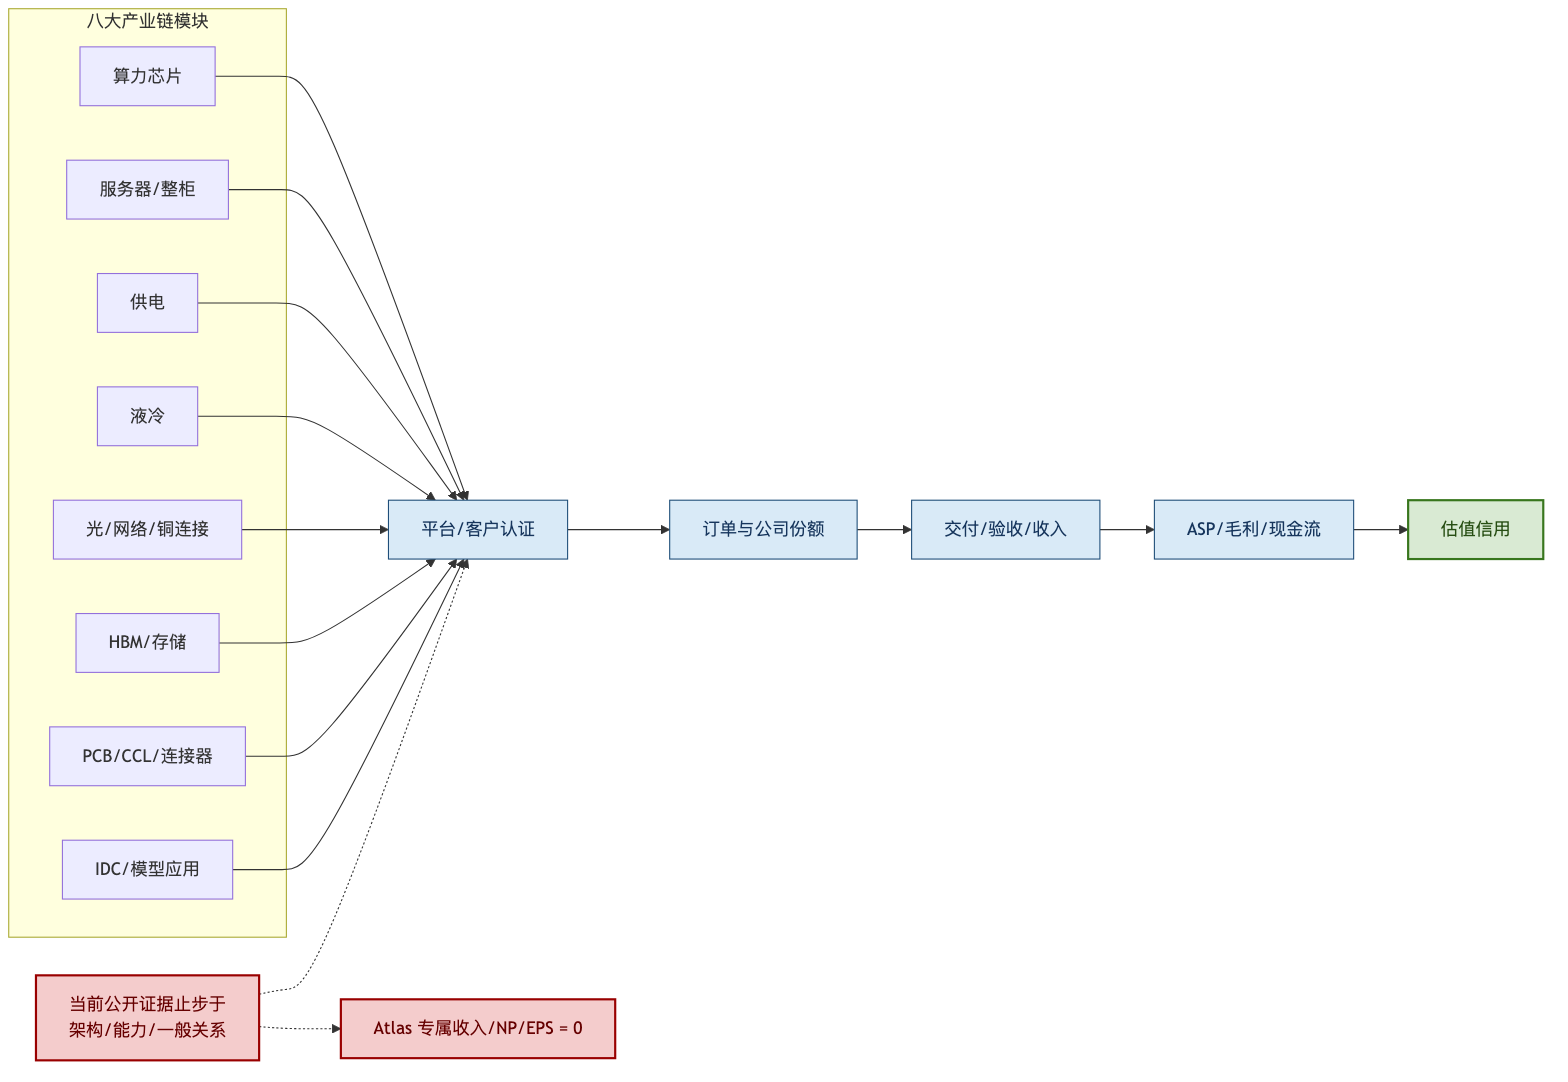
\includegraphics[width=\textwidth]{exhibits/chain_profit_gate.png}
\caption{八模块从架构能力到估值信用的证据闸门}
\sourcenote{AStock 产业链证据模型。任一环节缺少平台/客户、订单、验收或经济性，Atlas 专属盈利信用均维持为零。}
\end{figure}

该图解释了为什么“架构方向正确”和“公司可以估值”并不矛盾：12 家公司可凭已披露的更广义业务获得估值，但 Atlas 专属利润必须穿过四级闸门。目前上市公司证据大多停在能力或一般关系层，尚未抵达订单与公司份额。

\textbf{服务器、整柜与网络设备}是从芯片到可交付系统的第一层工程化价值。Atlas 950 最大设计包含 128 个计算柜和 32 个互联柜，涉及计算板、主控、BMC、机框、母线、功率组件、交换/网络柜、线缆、制造测试和现场服务。华为公开了模块、单板、卡和参考架构的伙伴开放方向，却没有披露 Atlas 950 的 OEM/ODM、机柜制造商、分工、ASP 或订单。神州数码、拓维信息等具有昇腾生态或服务器业务，但一个生态伙伴可能是分销、集成、品牌机或软件服务角色，收入纯度、毛利率和营运资金结构差异极大，必须拆开建模。四川长虹对投资者所称 AI 服务器 ODM 业务作出否认，因此被排除。

\textbf{光通信}是市场最容易过度线性外推的环节。全光 UB-Mesh 确认跨柜光互联的重要性，但没有端口数、模块速率、可插拔/LPO/CPO/OCS 路线、DSP 和光引擎规格。华工科技披露 2025 年光电器件收入 60.97 亿元、同比增长 53.39\%，并覆盖 800G、1.6T、3.2T、AEC/ACC 等产品，这是广义 AI 光连接能力和盈利基础；它没有披露 Atlas 平台认证或华为该项目订单。光迅科技、源杰科技、光库科技、长芯博创同样只能以产品与行业需求进入卫星池。若 UBoE 实际减少交换机/光模块数量，单纯按 8,192 卡乘历史模块比率反而会高估 TAM。

\textbf{PCB、CCL 与连接器/线缆}承载高速信号、电源、背板和整机互联。沪电股份、深南电路、胜宏科技、生益科技拥有明确的 AI 服务器、交换机、高速板或材料能力，2026H1 预告亦显示部分公司盈利高增长；但 Atlas 950 的板层、材料等级、正交无缆架构、连接器接口、良率、ASP 和供应商分配没有公开。航天电器具备高速背板与液冷连接能力，却没有确认投资者提问中的昇腾 950 关系；沃尔核材、兆龙互连、鼎通科技属于高速铜连接/连接器能力观察。能力越强，研究优先级越高；关系越不清晰，Atlas 估值信用仍为零。

\textbf{供配电与液冷}是多机柜超节点最明确的工程增量方向之一。Atlas 950 为全液冷系统，华为还披露浮动盲插液冷连接和材料/工艺协同。申菱环境的公开证据最接近“关系+产品”：完整年报原件披露华为为数据服务客户、与 H 公司合作，数据服务收入同比增长 51.42\%、新增订单约增长 72\%，并提供 CDU、Manifold、冷源、管网、快接和冷板；但仍没有点名 Atlas 950，也没有平台认证、订单、kW、ASP 和利润桥。英维克拥有从冷板、快接、Manifold、CDU 到冷源和工质的端到端能力，也披露部分主流芯片/设备厂商认可和规模采购，但没有华为 Atlas 分配。科华数据具备 200kW--1.5MW 液冷机组、40--120kW/柜 POD 等能力，并有昇腾创新中心案例；这些仍属于邻近项目证据。

\textbf{AIDC/IDC 运营}决定系统能否获得电力、站点、网络、PUE、水资源和持续利用率。运营商、云厂商、地方智算中心和模型公司是需求锚，不是上游订单证明。华为披露前代 384 卡系统的部署进展，却没有公布 Atlas 950 客户、站点和验收。科大讯飞与昇腾 950 协同开发证明下游工作负载需求，仍不能反推其采购 SuperPoD 的数量和成本；IDC 公司的资本开支也不能自动分配给某一服务器、液冷或光模块供应商。

\textbf{上游设备、材料与关键部件}是最重要、也最难公开验证的缺口。昇腾 950DT 的工艺、HBM 制造、先进封装和良率决定供给上限，出口管制又可能同时提升国产需求与限制设备/材料供给。市场常把探针卡、PCB 材料、液冷接头或光芯片能力直接映射到新平台，本报告要求至少出现“公司点名平台/产品+认证或订单+经济性”才升级。附录证据索引保留全部未证实节点、负面问答和下一条验证路径，避免只呈现支持性材料。

以上八段对应同一盈利传导逻辑：技术规格先形成潜在价值量，资格认证和订单决定公司份额，交付与客户验收决定收入确认，产品结构、良率和议价决定利润率，存货/应收/资本开支决定现金流，只有走完整条链条的利润才能获得估值信用。Atlas 950 当前只完成“系统实物展示”层，上市公司大多停在能力或关系层；因此本报告宁可保留覆盖缺口，也不把尚未发生的后半段写进 EPS。

\begin{exhibitbox}[八大产业链模块与 A 股定位]
\begin{longtable}{L{2.8cm}L{3.5cm}L{4.0cm}L{3.0cm}}
\toprule
\textbf{模块} & \textbf{Atlas 950 价值点} & \textbf{A 股/国内观察} & \textbf{当前证据结论}\\
\midrule
\endhead
算力与存储 & 950DT、HiZQ HBM、池化内存、AI 存储 & 科大讯飞为下游负载锚；国内芯片/存储相邻能力 & 制造、封装、HBM、良率和供应商未披露\\
服务器与整柜 & 计算柜、互联柜、BMC、整机制造服务 & 神州数码、拓维信息及国内服务器生态 & 伙伴关系不等于 Atlas OEM/ODM 订单\\
光网络与互联 & UB-Mesh、交换、光引擎、光纤、AEC/ACC & 华工科技、光迅科技及光器件公司 & 全光方向确认，模块数/规格/供应商未知\\
PCB/CCL & 高速高层板、背板、材料、封装基板 & 胜宏、沪电、深南、生益科技 & AI 能力/业绩强，Atlas 认证与规格未知\\
连接器与线缆 & 高速铜互联、盲插电/液连接、管路 & 沃尔、兆龙、鼎通、航天电器 & 能力可核验，平台关系未确认\\
供配电 & 变压器、UPS/HVDC、母线、PowerPOD & 科华数据、中恒电气、伊戈尔 & MW、拓扑、供应商与系统价值量未知\\
液冷与热管理 & 冷板、快接、Manifold、CDU、冷源 & 申菱、英维克、同飞股份 & 申菱关系最强；仍无 Atlas 专属订单\\
IDC/运营与应用 & 电力、站点、PUE、利用率、模型工作负载 & 运营商/云厂商；科大讯飞需求锚 & 需求有效，不可反推上游公司收入\\
\bottomrule
\end{longtable}
\sourcenote{50 节点全链条证据池、15 条公司关系记录、公司公告与华为官方资料；详见附录。}
\end{exhibitbox}

\section{利润池与护城河}

芯片与软件栈拥有最高价值密度，但也是供应和政策不透明度最高的环节；光互联、HBM 和先进封装技术壁垒高，盈利却对良率、代际和客户集中度敏感；服务器/整柜收入体量大但毛利率和营运资金通常较弱；供电与液冷经平台认证后生命周期较长，但可能被 OEM 内制或项目总包压缩利润；PCB/CCL/连接器的价值由材料等级、层数、良率和认证决定，名义产能不是利润；IDC/运营拥有稀缺电力和站点，但承担高折旧、债务和利用率爬坡。

在当前证据下，最稳妥的盈利映射不是猜“谁份额最大”，而是寻找已经在更广义 AIDC 业务中兑现收入、利润、订单和现金流的公司，再把 Atlas 作为 0 权重期权跟踪。这样即使最终供应链与传闻不同，估值仍有已披露业务支撑。

\section{公司关系升级规则}

能力观察升级为平台候选，至少需要公司或华为点名 Atlas/UnifiedBus/950 平台和具体产品；平台候选升级为订单候选，需要认证、定点、合同或在手订单；订单候选升级为盈利模型，需要数量/金额、交付与验收、收入拆分、毛利率或足够代理。任何一层缺失都在 coverage gap matrix 中保留下一验证路径，而不是以“有望”“深度受益”填补。
